\chapter{Implementace}


\section{Projekt}
Jak už bylo zmíněno v sekci architektura, aplikace nemá prezentační vrstvu a sestává se jenom z aplikačního serveru, který má na starosti komunikaci s klienty, byznys logiku a persistenci dat.
\par
Pro sestavení projektu je využit Maven, který nabízí jednoduché inkludování externích balíčků a také pluginy pro sestavování a nasazování aplikace. 

\subsection{Java EE}
Celý projekt je naimplementován v Javě EE verze 8. Ta obsahuje nové DateTime API, Streams API aj., dále například podporuje použití lambda výrazů, což zkracuje zápis a umožňuje například předávání funkcí. Tato funkcionalita byla využita při přijímaní požadavků \ref{lst:http} a kontrolování tokenů \ref{lst:token}. Dalším důležitým aspektem Javy EE jsou beany, které už byly představeny v sekci \ref{platforma} na tyto informace navážeme jejich anotacemi, které byly použity v rámci projektu. Většina bean je typu stateless, což znamená že si nepamatují stav napříč požadavky jednoho klienta, jenom po dobu jednoho daného požadavku, poté je objekt vrácen do poolu a může ho využít jiný klient. Dále je použita request scope beana, která je vytvořena s každým novým http požadavkem a není zničena dokud je požadavek aktivní. Objekt \textit{Starter}, který je použit pro prvotní procesy po naběhnutí aplikace a objekt \textit{PeriodicalCleaning}, který periodicky promazává nepotřebné soubory jsou typu Singleton. Což je beana, která je vytvořena jenom jednou a je globálně sdílená pro celou aplikaci. Byly využiti i jiné anotace a funkce, ale pro představu tyto stačí.

\subsection{Struktura pojektu}
Nyní si představíme strukturu projektu, tedy diagram baličků, který zobrazuje tři hlavní balíčky. První se jmenuje Api, který slouží pro zpracování požadavků (detailněji popsáno v sekci \ref{proRequests}), ten obsahuje tři další složky jmenovitě:
\begin{itemize}
	\item Controllers - Třídy zdrojů obsahující metody pro přijímání požadavků
	\item Responders - Třídy, které se starají o sestavování odpovědí klientům
	\item Contents - Třídy představující objekty pro serializaci a deserializaci JSON formátu
\end{itemize}
Další balíček v pořadí je Business, ten představuje všechnu logiku, která je aplikována na data. Nejdůležitejším balíčkem je Processes, ale zase si popíšeme všechny.
\begin{itemize}
	\item Services - Třídy obsahujicí hlavní logiku, tedy rozhodují co dělat s příchozímy daty
	\item Processes - Třídy pro kompilaci a úpravu PDF
	\item Entities - Třídy představující objekty používaní v aplikaci
\end{itemize}
Poslední se jmenuje Database a obsahuje tyto složky:
\begin{itemize}
	\item Sessions - Třídy pro komunikaci s databází 
	\item MyBatis - Třídy pro mapování SQL dotazů a nastavování spojení
\end{itemize}

\begin{figure}[H]
	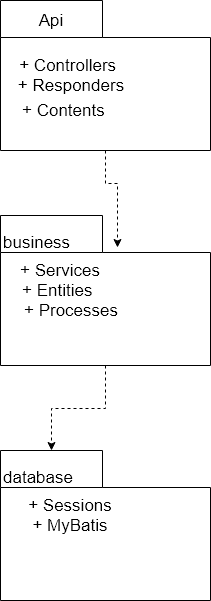
\includegraphics[scale=0.5]{packages}
	\centering
	\caption{Diagram balíčků}
	\label{fig:pack}
\end{figure}

Projekt obsahuje i další nevyobrazené balíčky, ale ty jsou spíše pomocné a tudíž nejsou tak důležité z pohledu funkčnosti a průchodu aplikací např. Utils, Exceptions, Enums, atd.

\subsection{Diagram tříd}
Na ukázku byly vytvořeny dva diagramy tříd, ty popisují jejich provázanost. První diagram \ref{fig:packResp} ukazuje hierarchii, kde úplně nahoře je obecná abstraktní třída, která má například metodu \textit{processRequest}, která je popsána v sekci\ref{proRequests}. Pod ní je třída \textit{EntityResponder}, která je také abstraktní a navíc generická, ta představuje už konkrétnější skupinu s metodami pro parsování JSON do objektů daných typem a naopak. Od ní dědí v našem případě dvě třídy, \textit{JobResponder} vytváří odpovědi pro žádosti na adresu /job a \textit{AppResponder} na adrese /app. 

\begin{figure}[H]
	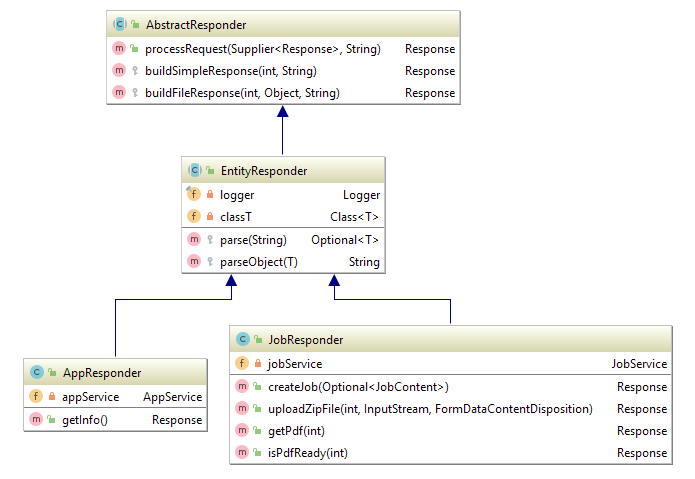
\includegraphics[scale=0.7]{packageResp}
	\centering
	\caption{Diagram tříd balíčku Responders}
	\label{fig:packResp}
\end{figure}

Na druhém diagramu \ref{fig:packProc} je vidět jaké třídy se hlavně starají o kompilaci a editaci. Všechny kromě \textit{ProcessUtils}, která jenom poskytuje metodu pro samotnou exekuci příkazů, implementují rozhraní \textit{Process} s metodou \textit{runProcess}. Ta je jediná která by měla být v jednotlivých třídách volána, představuje proběhnutí požadovaného procesu se vším všudy. V našem případě je nejdříve volána metoda z třídy \textit{MainProcess} a ta následně zajistí kompilaci a úpravu za pomoci vyobrazených tříd \textit{CompileProcess} a \textit{EditProcess}.
\newpage
\begin{figure}[H]
	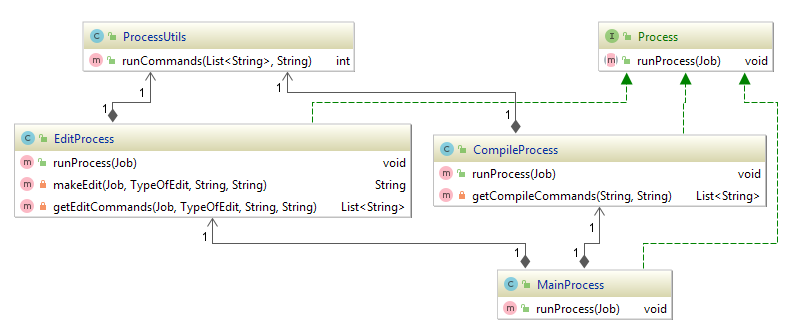
\includegraphics[scale=0.7]{packageProc}
	\centering
	\caption{Diagram tříd týkajicí se balíčku Processes}
	\label{fig:packProc}
\end{figure}


\section{Aplikační server}
V této sekci hlavně rozebereme nastavení serveru. Je použita Payara ve verzi 191 Full, ale dále zmiňované nastavení není nijak zavislé na verzi. Bohužel jsem nebyl schopen nastavit JDBC pool v Payaře, což ale bylo vyřešeno jiným způsobem popsaným v sekci \ref{sqlite}. Byly přidány čtyři JNDI zdroje pro nastavení cesty k hlavnímu adresáři, cesty k souboru s databází a cest ke spustitelným souborům programů MikTeX a PDFtk. Nic jiného k úspěšnému spuštění aplikace není potřeba.

\section{Zpracovávání požadavků} \label{proRequests}
Požadavky klienta jsou přijímány skrze REST Api, jak můžeme vidět na ukázce \ref{lst:http}, kde je vyobrazena funkce, která reaguje na htttp požadavek typu POST na základní adrese /job. Přijímá data ve formátu JSON, které obsahují požadavky na výsledné PDF, ale také token, použivaný k autentizaci.    

\begin{lstlisting}[caption=Funkce pro přijímání HTTP požadavků, label={lst:http}]
@POST
@Consumes(MediaType.APPLICATION_JSON)
public Response postJob(@QueryParam("token") String token, String data) {
 return jobResponder.processRequest(() 
			-> jobResponder.createJob(data), token);
}
\end{lstlisting} 

Token je zkontrolován ve funkci \textit{processRequest} \ref{lst:token}, ta kromě tokenu přijimá i parametr Supplier<Response>, který představuje obecnou funkci bez parametru s návratovou hodnotou typu Response. Tudíž se jako první zkontroluje daný token, pokud je nesprávný je rovnou vrácena odpověď UNAUTHORIZED v opačném případě je zavolána předaná funkce pomocí metody \textit{get()}, kterou definuje interface Supplier.   
\newpage
\begin{lstlisting}[caption=Funkce na ověření tokenu v požadavku, label={lst:token}]
public Response processRequest(Supplier<Response> request, String token) {
 Response response = null;
 if (TokenUtils.checkToken(token)) {
  response = request.get();
 } else {
  response = buildSimpleResponse(401, "Bad token");
 }
 return response;
}
\end{lstlisting}

Následuje objekt typu Responder, která se stará o sestavování odpovědí klientovi na základě vyjímek či výstupů ze servisní vrstvy. Ta obsahuje logiku aplikace, na základě typu požadavku, buď data persistentně uloží nebo například započne hlavní proces služby, tedy kompilaci. O ukládání dat se starají Session objekty, které si získají spojení s databází a vykonají daný SQL dotaz.

\section{Kompilace a úprava PDF}
Jak bylo uvedeno v návrhu (sekce \ref{compilation}), pro kompilování \LaTeX\ souborů je vybrán \textbf{MikTeX}, ten je potřeba nejdříve nainstalovat v příslušné konfiguraci, která byla popsána v téže sekci, vybraná verze je 2.9.7. Samotná kompilace je prováděna pomocí PdfLatex, ten je spouštěn s těmito parametry: 
\begin{itemize}
	\item interaction = nonstopmode - program nečeká na vstup
	\item include-directory - slouží k určení adresáře, kde se nachází tex soubory
	\item output-directory - adresář pro výstupní PDF soubor
	\item aux-directory - adresář pro ostatní výstupní soubory, jako jsou logy
	\item jméno hlavního tex souboru
\end{itemize}
Výstupem je tedy soubor PDF, na který je potřeba ještě aplikovat požadavky od klienta.
K tomu je použit program \textbf{PDFtk} verze 2.02. Pro požadované úpravy jsou potřeba tyto argumenty:
\begin{itemize}
	\item output - určuje výstupní adresář
	\item cat - spojuje dva PDF soubory dohromady
	\item background - přidává vodoznak
	\item owner\_pw a user\_pw - první nastavuje heslo vlastníka a druhý heslo uživatele\footnote{Rozdíl je popsán v kapitole \ref{PDF}}
	\item allow copycontents - umožňuje kopírovat text
	\item allow printing - povoluje tisk
\end{itemize}
Jelikož se argumenty kromě output, allow copycontents a printing nedají řetězit, je každá úpráva vykonávána samostatně. Pro lepší představu následuje ukázka právě zaheslování a přidání práv pro kopírování a tisk.

\begin{lstlisting}[caption=Zaheslování a úprava práv souboru PDF]
 commands.addAll(Arrays.asList("output", directoryPath + outputFileDir);
 commands.addAll(Arrays.asList("owner_pw", job.getPassword()));
 commands.addAll(Arrays.asList("user_pw", String.valueOf(job.hashCode())));
 if (job.isCopyable() || job.isPrintable()) {
  commands.add("allow");
 }
 if (job.isCopyable()) {
  commands.add("copycontents");
 }
 if (job.isPrintable()) {
  commands.add("printing");
 }
\end{lstlisting}

Můžeme vidět, že nejdříve se nastaví argument output, dále se nastavuje heslo vlastníka, to byl přijmuto od klienta, naopak jako heslo uživatele se použije vygenerovaný hash, který zajišťuje dostatečnou bezpečnost a náhodnost. Jestliže si uživatel přál kopírovatelnost a tisknutelnost je přidán argument allow a za ním dané povolení, buď jedno nebo obě.

\subsection{Vykonávání příkazů}
Java poskytuje rozhraní pro spouštění procesů a zacházení s nimi. Nejdříve je potřeba ProcessBuilderu předat pole stringů, kde první je název nebo cesta ke spustitelnému souboru a ostatní jsou argumenty daného příkazu. Zavoláním metody start na právě vytvořeném objektu, získáme objekt Process, který už představuje běžící proces definovaný zadanými argumenty. Nyní je možné číst výstupy(normální i chybový) programu, ale je i umožněno psaní na vstup. Metoda \textit{waitFor} čeká na dokončení procesu a její návratová hodnota udává zda-li byl program ukončen chybou nebo normálním způsobem.   
\begin{lstlisting}[caption=Metoda pro spuštění procesu]
 public int runCommands(List<String> commands, String logName) {
  Process process = new ProcessBuilder(commands).start();
  InputStream is = process.getInputStream();
  BufferedReader reader = new BufferedReader(new InputStreamReader(is));
  
  String logFile = directoryPath + DirUtils.LOG_DIR + logName + ".txt";
  BufferedWriter log = new BufferedWriter(new FileWriter(logFile));
  
  String line;
  while ((line = reader.readLine()) != null) {
    log.write(line + System.lineSeparator());
  }
  log.flush();
  log.close();
  return process.waitFor();
 }
\end{lstlisting}

Tato ukázka kódu představuje zmiňované zacházení s procesy používané pro kompilaci a úpravu do PDF, kde výstup programu je vypisován do textového souboru, pro budoucí použití.

\section{Ukládání dat}
Data jsou ukládána několika způsoby za prvé se využívá databáze do které se ukládají požadavky klienta na výsledné PDF. Dále se použivájí již zmíněné properties soubory v kterých se nachází tokeny. A v neposlední řadě se všechny vygenerované PDF ukládají do klasického souborového systému. 
\begin{figure}[H]
	\centering
	\begin{minipage}{15cm}
		\dirtree{%
			.1 /.
			.2 app.  
			.3 log \ldots{} \begin{minipage}[t]{10cm}
				logy pro potřeby aplikace
			\end{minipage}.
			.2 archive \ldots{} \begin{minipage}[t]{5cm}
				zazipované archivy
			\end{minipage}.
			.2 pdf.
			.3 final \ldots{} \begin{minipage}[t]{5cm}
				výsledné PDF
			\end{minipage}.
			.3 postcompile \ldots{} \begin{minipage}[t]{5cm}
				PDF před úpravami
			\end{minipage}.
			.3 temp \ldots{} \begin{minipage}[t]{8cm}
				pomocná složka pro úpravy
			\end{minipage}.
			.2 latex.
			.3 aux \ldots{} \begin{minipage}[t]{8cm}
				ostatní výstupní soubory kompilace
			\end{minipage}.
			.2 log \ldots{} \begin{minipage}[t]{5cm}
				logy z kompilace a úprav
			\end{minipage}.
		}
	\end{minipage}
	\caption{Adresářový strom}
	\label{fig:dirs}
\end{figure}
Na obrázku \ref{fig:dirs} můžeme vidět adresářovou strukturu s popisem k čemu dané složky slouží. 

\subsection{SQLite a MyBatis} \label{sqlite}
\paragraph{SQLite}
Tato databáze staví na klasickém SQL jazyku a stejně jako všechny ostatní nejznámější databáze i tato je relačním. Ovšem narozdíl od ostatních nepotřebuje ke svému běhu server, pouze vytváří databáze v podobě souborů na disku, ke kterým poskytuje rozhraní knihovna SQLite JDBC. Použitá verze JDBC v této práci je 3.27.2.1. Tato datábaze má velmi omezený počet typů například neobsahuje boolean, což bylo vyřešeno pomocí mapování frameworkem MyBatis\footnote{http://www.mybatis.org/mybatis-3/}, který je popsán o odstavec níže. Pomohl také k vyřešení problému ohledně JDBC poolu, který nešel nastavit v aplikačním serveru.

\paragraph{MyBatis} 
Je knihovna pomocí, která umožňuje mapování databáze na entity, předdefinovat si SQL dotazy a komunikovat se samotnou databází. Je použita ve verzi 3.5.0. Hlavní výhodou je velká customizace, která je potřeba při zacházení s SQLite, jak už bylo napsáno výše, bylo vytvořeno mapování z typu boolean na typ integer a naopak. Dále dokáže spravovat spojení s databází, je možné nastavit pooling atd. Nastavení mapování entit a dotazů a samotná konfigurace se píše do XML souborů. Kde byl například nastaven již zmíněný JDBC pool, to vše je vidět v ukázce níže \ref{lst:jdbc}.

\begin{lstlisting}[caption=Konfigurace JDBC poolu, label={lst:jdbc}]
<environment id="development">
 <transactionManager type="JDBC"/>
 <dataSource type="POOLED">
  <property name="driver" value="org.sqlite.JDBC"/>
  <property name="url" value="${url}"/>
 </dataSource>
</environment>
\end{lstlisting}
